% Problem 1 - Impedance conversion table (12 points)
\Point{impedanceforms}{filltable}{12}
\begin{mainquestion}{impedanceforms}{Impedance Conversion Table}

\begin{partquestion}{filltable}{Fill out the following table. Assume an angular frequency of \qty{1}{\radian/\second}}
% Imported from a solutions document. The prompt table below is reconstructed with only the given Cartesian impedances populated.

{\small
\renewcommand{\arraystretch}{1.25}
\begin{center}
\resizebox{\textwidth}{!}{%
\begin{tabular}{|c|c|c|c|c|c|c|c|c|c|}
\hline
Cartesian form of $Z$ & Polar form of $Z$ & Euler form of $Z$ & Series equivalent circuit for $Z$ & Parallel equivalent circuit for $Z$ & Admittance & Resistance & Reactance & Conductance & Susceptance \\
\hline
$1 + 2j\ \Omega$ & & & & & & & & & \\
\hline
$1.5 + 1.5\sqrt{3}j\ \Omega$ & & & & & & & & & \\
\hline
$2\sqrt{2} - 2\sqrt{2}j\ \Omega$ & & & & & & & & & \\
\hline
$5 - \frac{1}{6}j\ \Omega$ & & & & & & & & & \\
\hline
$3.965 + 3.469j\ \Omega$ & & & & & & & & & \\
\hline
$\frac{3}{25} - \frac{4}{25}j\ \Omega$ & & & & & & & & & \\
\hline
\end{tabular}%
}
\end{center}
}

\begin{answer}
{\small
\renewcommand{\arraystretch}{1.25}
\begin{center}
\resizebox{\textwidth}{!}{%
\begin{tabular}{|c|c|c|c|c|c|c|c|c|c|}
\hline
Cartesian form of $Z$ & Polar form of $Z$ & Euler form of $Z$ & Series equivalent circuit for $Z$ & Parallel equivalent circuit for $Z$ & Admittance & Resistance & Reactance & Conductance & Susceptance \\
\hline
$1 + 2j\ \Omega$ & $\sqrt{5}\angle 63.43^{\circ}$ & $\sqrt{5}e^{j\tan^{-1}(2)}$ & 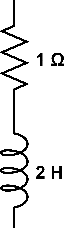
\includegraphics[height=0.95in]{questionbank/circuit_quantities/impedance_forms/v0/row1_series.png} & 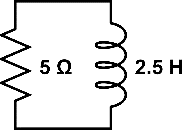
\includegraphics[height=0.6in]{questionbank/circuit_quantities/impedance_forms/v0/row1_parallel.png} & $0.2 - 0.4j\text{ S}$ & $1\ \Omega$ & $2\ \Omega$ & $0.2\text{ S}$ & $-0.4\text{ S}$ \\
\hline
$1.5 + 1.5\sqrt{3}j\ \Omega$ & $3\angle 60^{\circ}$ & $3e^{j\frac{\pi}{3}}$ & 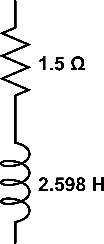
\includegraphics[height=0.95in]{questionbank/circuit_quantities/impedance_forms/v0/row2_series.png} & 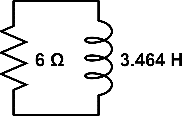
\includegraphics[height=0.6in]{questionbank/circuit_quantities/impedance_forms/v0/row2_parallel.png} & $\frac{1}{6} - \frac{\sqrt{3}}{6}j\text{ S}$ & $1.5\ \Omega$ & $1.5\sqrt{3}\ \Omega$ & $\frac{1}{6}\text{ S}$ & $-\frac{\sqrt{3}}{6}\text{ S}$ \\
\hline
$2\sqrt{2} - 2\sqrt{2}j\ \Omega$ & $4\angle -45^{\circ}$ & $4e^{-j\frac{\pi}{4}}$ & 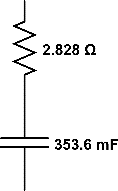
\includegraphics[height=0.95in]{questionbank/circuit_quantities/impedance_forms/v0/row3_series.png} & 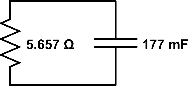
\includegraphics[height=0.6in]{questionbank/circuit_quantities/impedance_forms/v0/row3_parallel.png} & $\frac{\sqrt{2}}{8} + \frac{\sqrt{2}}{8}j\text{ S}$ & $2\sqrt{2}\ \Omega$ & $-2\sqrt{2}\ \Omega$ & $\frac{\sqrt{2}}{8}\text{ S}$ & $\frac{\sqrt{2}}{8}\text{ S}$ \\
\hline
$5 - \frac{1}{6}j\ \Omega$ & $5.003\angle -1.9^{\circ}$ & $5.003e^{j\tan^{-1}\left(-\frac{1}{30}\right)}$ & 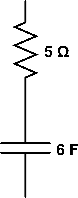
\includegraphics[height=0.95in]{questionbank/circuit_quantities/impedance_forms/v0/row4_series.png} & 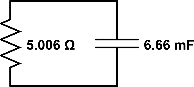
\includegraphics[height=0.6in]{questionbank/circuit_quantities/impedance_forms/v0/row4_parallel.png} & $0.200 + 0.0067j\text{ S}$ & $5\ \Omega$ & $-\frac{1}{6}\Omega$ & $0.200\text{ S}$ & $0.0067\text{ S}$ \\
\hline
$3.965 + 3.469j\ \Omega$ & $5.27\angle 41.2^{\circ}$ & $5.27e^{j(0.719)}$ & 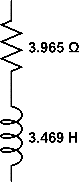
\includegraphics[height=0.95in]{questionbank/circuit_quantities/impedance_forms/v0/row5_series.png} & 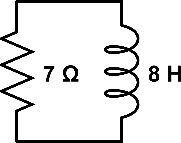
\includegraphics[height=0.6in]{questionbank/circuit_quantities/impedance_forms/v0/row5_parallel.png} & $0.143 - 0.125j\text{ S}$ & $3.965\ \Omega$ & $3.469\ \Omega$ & $0.143\text{ S}$ & $-0.125\text{ S}$ \\
\hline
$\frac{3}{25} - \frac{4}{25}j\ \Omega$ & $0.2\angle -53.1^{\circ}$ & $0.2e^{-j(0.927)}$ & 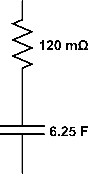
\includegraphics[height=0.95in]{questionbank/circuit_quantities/impedance_forms/v0/row6_series.png} & 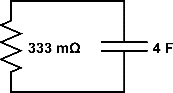
\includegraphics[height=0.6in]{questionbank/circuit_quantities/impedance_forms/v0/row6_parallel.png} & $3 + 4j\text{ S}$ & $\frac{3}{25}\ \Omega$ & $-\frac{4}{25}\ \Omega$ & $3\text{ S}$ & $4\text{ S}$ \\
\hline
\end{tabular}%
}
\end{center}
}

To convert in general, starting with a Cartesian form of $Z = a + jb$, the polar form will be $\sqrt{a^{2} + b^{2}}\angle\tan^{-1}\left(\frac{b}{a}\right)$, and Euler's form is $\sqrt{a^{2} + b^{2}}e^{j\tan^{-1}\left(\frac{b}{a}\right)}$. The serial equivalent circuit will be a resistor of value $a$ and an inductor of value $b$ if $b > 0$, or a capacitor of value $-\frac{1}{b}$ if $b < 0$. The parallel equivalent circuit will be a resistor of value $\frac{a^{2} + b^{2}}{a}$ and an inductor of value $\frac{a^{2} + b^{2}}{b}$ if $b > 0$, or a capacitor of value $-\frac{b}{a^{2} + b^{2}}$ if $b < 0$. The admittance is
\[
\frac{1}{a + jb} = \frac{a - jb}{a^{2} + b^{2}} = \frac{a}{a^{2} + b^{2}} - j\frac{b}{a^{2} + b^{2}}
\]
(compare with the parallel equivalent circuit). From here, the resistance is $a$, the reactance is $b$, the conductance is $\frac{a}{a^{2} + b^{2}}$ and the susceptance is $\frac{-b}{a^{2} + b^{2}}$.
Starting with any of the first six columns, you can work out the other entries based on the relationships described above.
\end{answer}
\end{partquestion}

\end{mainquestion}

% Problem 2 - Complex gain at a single frequency (10 points)
\clearpage
\Point{singlefreqgain}{complexforms}{3}
\Point{singlefreqgain}{outputwaveform}{5}
\Point{singlefreqgain}{otherfrequencies}{2}
\begin{mainquestion}{singlefreqgain}{Complex Gain at a Single Frequency}

A black box with an input and output is found to have a voltage gain magnitude $\left|H\left(j\omega_{0}\right)\right| = 17$ at a frequency $\omega_{0}$, with $v_{o}(t)$ leading $v_{i}(t)$ by $17^{\circ}$ (both voltages are assumed to be sinusoids).

\begin{partquestion}{complexforms}{Express the gain at $\omega_{0}$ as a complex number in both Cartesian and Euler forms. Be careful with your degrees and radians!}
\begin{answer}
The problem describes a voltage gain $H(j\omega)$ at a specific frequency $\omega_{0}$:

\[
H\left(j\omega_{0}\right) = 17e^{j2\pi\left(\frac{17}{360}\right)} = 17e^{j(0.297)}
\]

In Cartesian form, it becomes:

\begin{align*}
H\left(j\omega_{0}\right) &= 17\cos\left(0.297\right)+j17\sin\left(0.297\right)\\
&= 16.26+4.97j
\end{align*}

\end{answer}
\end{partquestion}

\begin{partquestion}{outputwaveform}{Find an expression for $v_{o}(t)$ at $\omega_{0}$ assuming $v_{i}(t) = \cos\left(\omega_{0}t - 17^{\circ}\right)$. Sketch both input and output waveforms vs. time, on the same set of axes.}
\begin{answer}
Using Euler's notation, we have:

\[
\mathbf{V_{\it{i}}} = e^{j\left(\omega_{0}t - 2\pi\left(\frac{17}{360}\right)\right)}
\]

so
\begin{align*}
\mathbf{V_{\it{o}}} &= \mathbf{V_{\it{i}}}H\left(j\omega\right)\\
&=17e^{j\left(\omega_{0}t + 2\pi\left(-\frac{17}{360}+\frac{17}{360}\right)\right)}\\
&=17e^{j\omega_{0}t}
\end{align*}

This implies that $v_{o}(t) = 17\cos\left(\omega_{0}t\right)$.

\begin{center}
    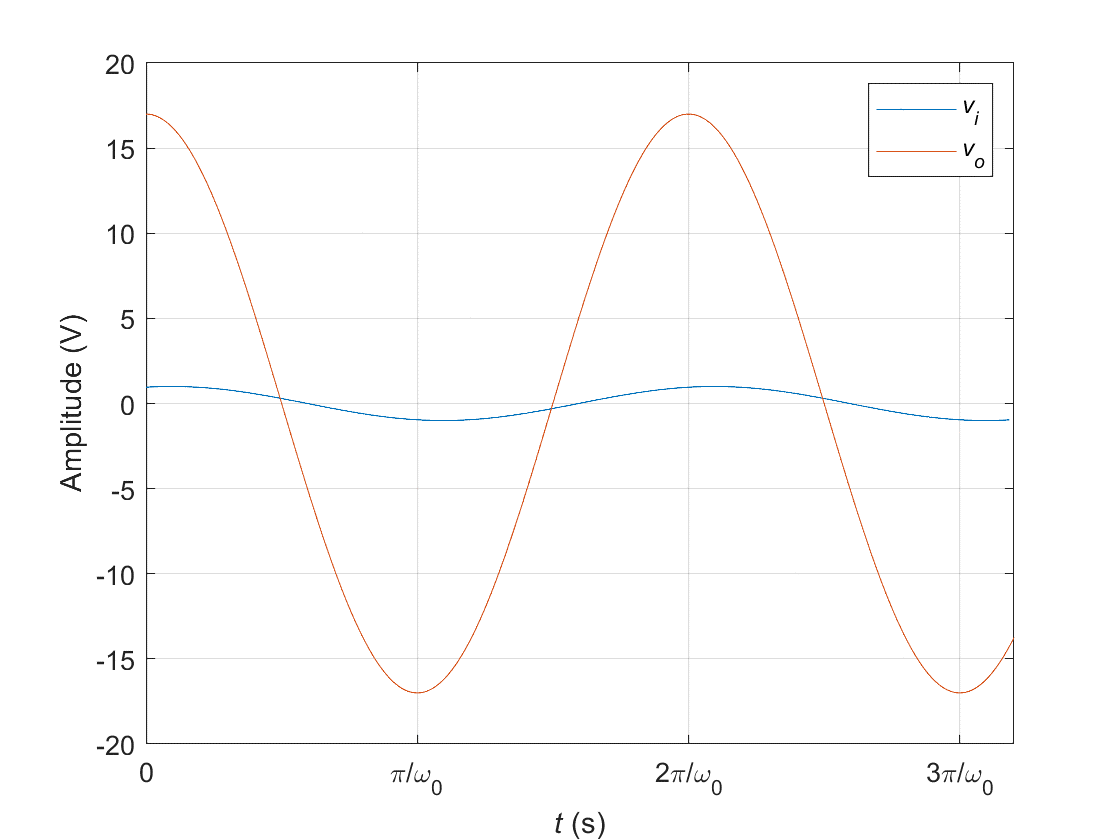
\includegraphics[width=5.2in]{questionbank/networks/single_frequency_gain/v0/waveforms.png}
\end{center}
\end{answer}
\end{partquestion}

\begin{partquestion}{otherfrequencies}{What can we say about the gain at $2\omega_{0}$? What about $\frac{1}{2}\omega_{0}$?}
\begin{answer}
Absolutely nothing, for either! We are only given information about the gain at one frequency, namely $\omega_{0}$. It is entirely unspecified for any other frequency of consideration.
\end{answer}
\end{partquestion}

\end{mainquestion}

% Problem 3 - Bridge-circuit RC filter (16 points)
\clearpage
\Point{bridgefilter}{transferfunction}{5}
\Point{bridgefilter}{functionality}{1}
\Point{bridgefilter}{bodesketch}{4}
\Point{bridgefilter}{cornerfrequency}{2}
\Point{bridgefilter}{outputvoltage}{4}
\begin{mainquestion}{bridgefilter}{Bridge-Circuit RC Filter}

Consider the bridge circuit shown on the right.

\begin{center}
    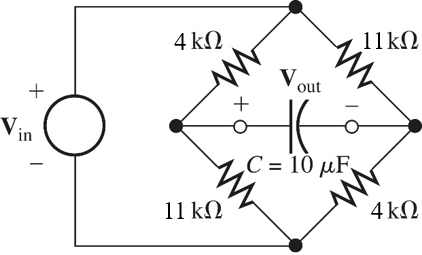
\includegraphics[width=4.3in]{questionbank/networks/bridge_rc_filter/v0/bridge_circuit.png}
\end{center}

\begin{partquestion}{transferfunction}{Find the transfer function $H\left(j\omega\right) = \frac{\mathbf{V_{\text{out}}}}{\mathbf{V_{\text{in}}}}$ of the circuit. \textit{Hint: Find a Th\'evenin equivalent for the circuit seen by the capacitor.}}
\begin{answer}
To find the Th\'evenin resistance, we short the voltage source and look into the circuit from the perspective of the capacitor. With the voltage shorted, the potential at the top node of the circuit is the same as that of the bottom node---they are thus the same node. So the resistance is just:
\begin{align*}
R_{\mathrm{th}}&=\left(\qty{4}{\kilo\ohm}||\qty{11}{\kilo\ohm}\right)+\left(\qty{4}{\kilo\ohm}||\qty{11}{\kilo\ohm}\right)\\
&=2\frac{(4)(11)}{4+11}\\
&=\frac{88}{15} \qty{ }{\kilo\ohm}
\end{align*}

To find the Thevenin (open-circuit) voltage, we remove the capacitor and notice that it will be just the difference between two voltage dividers:
\begin{align*}
\mathbf{V_{th}} &= \frac{11}{4+11}\mathbf{V_{in}}- \frac{4}{4+11}\mathbf{V_{in}}\\
&=\frac{7}{15}\mathbf{V_{in}}
\end{align*}


We can write the equivalent circuit as follows:

\begin{center}
    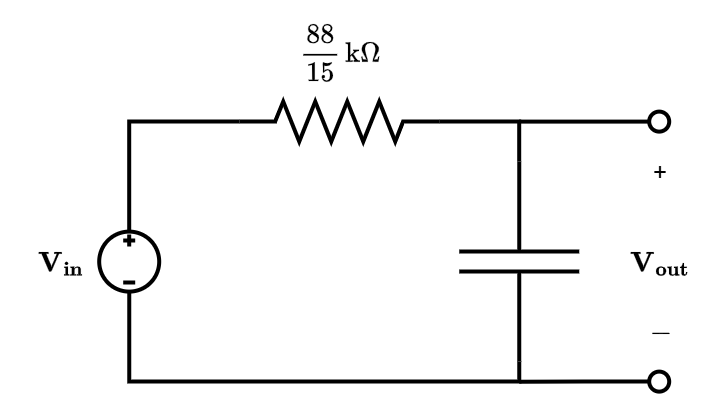
\includegraphics[width=4.8in]{questionbank/networks/bridge_rc_filter/v0/thevenin_equivalent.png}
\end{center}

From here, we can directly write the transfer function as a voltage divider with complex impedances:
\begin{align*}
H\left(j\omega\right) &= \frac{\mathbf{V_{\text{out}}}}{\mathbf{V_{\text{in}}}}\\
&=\left(\frac{7}{15}\right)\frac{\frac{1}{j\omega C}}{(R+\frac{1}{j\omega C}}\\
&=\frac{\frac{7}{15}}{1+j\omega RC}\\
&=\frac{\frac{7}{15}}{1+j\omega\left(\frac{88}{15}\times10^3\right)\left(10\times10^{-6}\right)}\\
&=\frac{\frac{7}{15}}{1+j\omega\left(\frac{22}{375}\right)}\\
&=\frac{175}{375+j22\omega}
\end{align*}
\end{answer}
\end{partquestion}

\begin{partquestion}{functionality}{Based on the result from (a), identify the functionality of this circuit (what does it do?)}
\begin{answer}
This is a low pass filter.
\end{answer}
\end{partquestion}

\begin{partquestion}{bodesketch}{Plot a sketch (to scale) of $\left|H\left(j\omega\right)\right|$ and $\angle H\left(j\omega\right)$.}
\begin{answer}
The magnitude is:

\begin{center}
    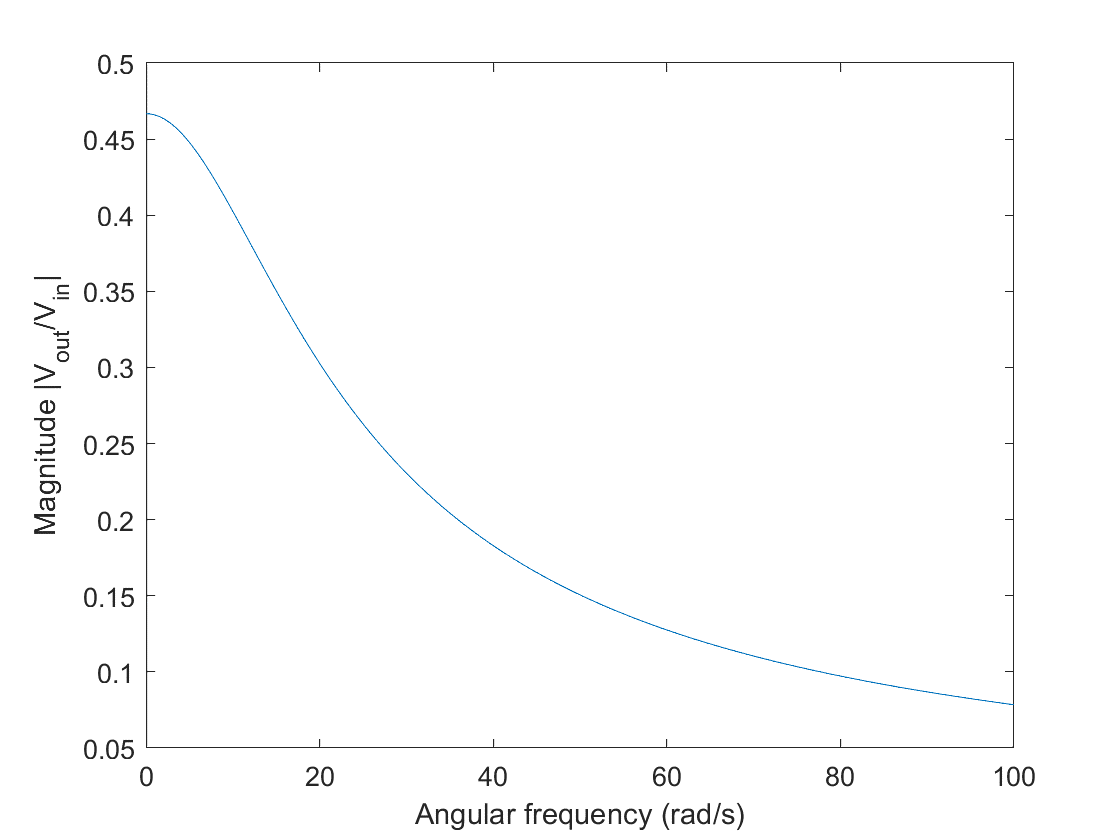
\includegraphics[width=5.3in]{questionbank/networks/bridge_rc_filter/v0/magnitude_plot.png}
\end{center}

The phase is:

\begin{center}
    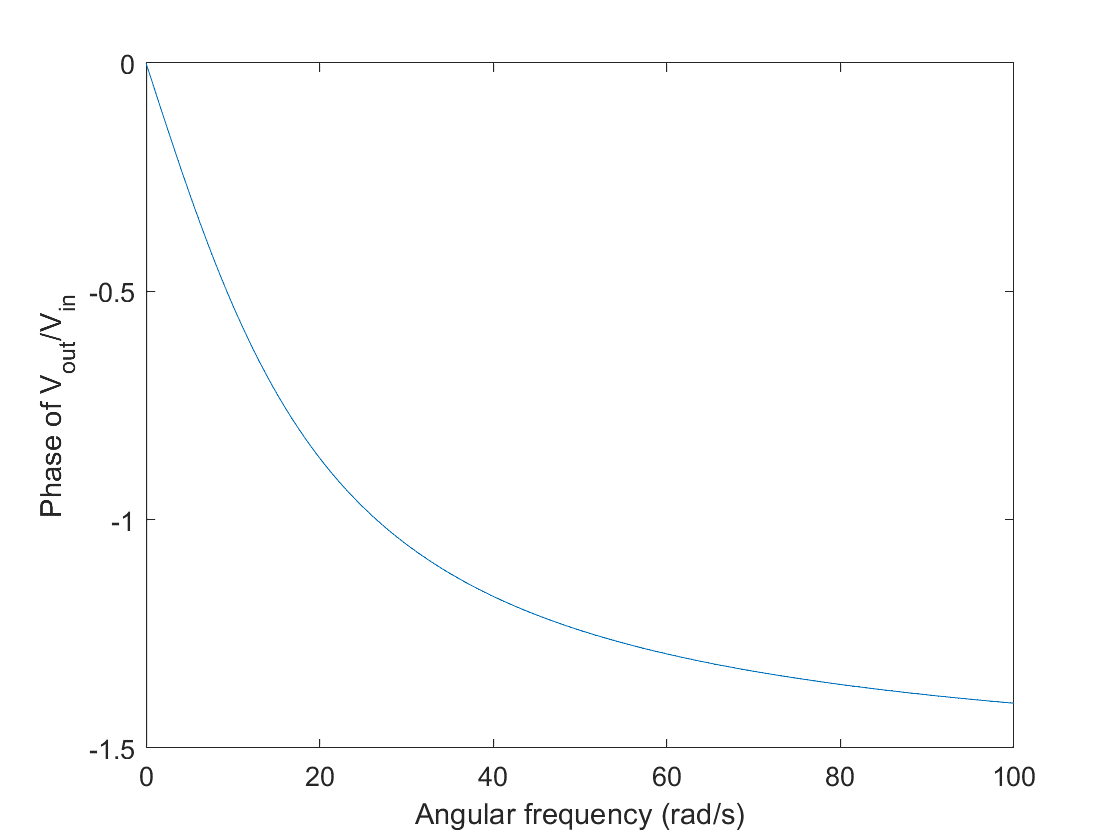
\includegraphics[width=5.3in]{questionbank/networks/bridge_rc_filter/v0/phase_plot.png}
\end{center}
\end{answer}
\end{partquestion}

\begin{partquestion}{cornerfrequency}{What is the corner frequency $\omega_{c}$?}
\begin{answer}
% NOTE: The imported source appears numerically inconsistent with the surrounding circuit and plots. Preserved here for manual review.
We can either estimate it from the graph by finding the angular frequency where the magnitude is 0.707 times the peak value, or we can calculate it directly from the expression for the transfer function. Either way, we should get a similar value: $\omega_{c} = \frac{1}{RC} = \frac{1}{5.867 \times 10^{-2}} = \qty{17}{\radian/\second}$
\end{answer}
\end{partquestion}

\begin{partquestion}{outputvoltage}{What is the output voltage if the input voltage is $v_{i}(t) = 2 + 3\sin\left(\omega_{c}t\right) + 4\sin\left(2\omega_{c}t\right)$?}
\begin{answer}
% NOTE: The final imported expression appears to contain OCR inconsistencies. Preserved here for manual review.
We need to determine the gain and phase of the transfer function for three separate frequencies: DC, the corner frequency, and twice the corner frequency. At DC, the gain is $\frac{7}{15}$ and there is no phase shift, so we will see an output of $2\left(\frac{7}{15}\right) = \frac{14}{15}\text{ V}$ from the DC term. At $\omega_{c}$, there is a gain of $\frac{7}{15}\left(\frac{1}{\sqrt{2}}\right) \approx 0.330$ and a phase shift of $-45^{\circ}$, so we will see an output of $3(0.330)\sin\left(\omega_{c}t - 45^{\circ}\right) = 0.990\sin\left(\omega_{c}t - 45^{\circ}\right)\text{ V}$ from the $\omega_{c}$ component of the input. Looking at the graphs at $2\omega_{c}$, there is a gain of about $0.210$ and a phase shift of about $-63.3^{\circ}$, so we will see an output of $4(0.210)\sin\left(2\omega_{c}t - 63.3^{\circ}\right) = 0.839\sin\left(2\omega_{c}t - 63.3^{\circ}\right)\text{ V}$ from the $2\omega_{c}$ component of the input. Putting this all together, we have:

\[
v_{o}(t) = \frac{14}{15} + 0.990\sin\left(\omega_{c}t - 45^{\circ}\right) + 0.839\sin\left(2\omega_{c}t - 63.3^{\circ}\right)\text{ V.}
\]
\end{answer}
\end{partquestion}

\end{mainquestion}

% Problem 4 - RL high-pass design (10 points)
\clearpage
\Point{rlhighpass}{cornerfrequency}{3}
\Point{rlhighpass}{inductance}{2}
\Point{rlhighpass}{bodeplots}{5}
\begin{mainquestion}{rlhighpass}{RL High-Pass Filter Design}

Suppose you are tasked with attenuating a 60 Hz input component signal by a factor of 100 using an $RL$ high-pass circuit.

\begin{partquestion}{cornerfrequency}{What is the corner frequency $f_{c}$? How does this corner frequency relate to the time constant $\tau$ for an $RL$ circuit?}
\begin{answer}
We want the input to be reduced by a factor of 100, which in decibels is $-20\log 100 = -20(2) = -40\text{ dB}$. Using the asymptotic Bode approximation, the high-pass circuit will have a roll-off at $-20$ dB/decade from the corner frequency, so the corner frequency must be 2 decades above 60 Hz, namely:

\[
f_{c} = \left(60\text{ Hz}\right)\left(100\right) = 6\text{ kHz.}
\]

Since $\omega_{c} = 2\pi f_{c} = \frac{R}{L} = \frac{1}{\tau}$, it follows that:

\[
f_{c} = \frac{1}{2\pi\tau}.
\]
\end{answer}
\end{partquestion}

\begin{partquestion}{inductance}{You wish to design this circuit, and of course you have on hand a 17 k$\Omega$ resistor for the job. What is the necessary value of $L$?}
\begin{answer}
Since $2\pi f_{c} = \frac{R}{L}$, we can solve for $L$ and find:

\[
L = \frac{R}{2\pi f_{c}} = \frac{17\text{ k}\Omega}{2\pi\left(6\text{ kHz}\right)} = 0.451\text{ H.}
\]
\end{answer}
\end{partquestion}

\begin{partquestion}{bodeplots}{Draw the Bode plots (both magnitude and phase) of the transfer function $H\left(j\omega\right) = \frac{\mathbf{V_{\text{out}}}}{\mathbf{V_{\text{in}}}}$ for this high-pass filter.}
\begin{answer}
Since the transfer function of the high pass RL filter is:

\[
H\left(j\omega\right) = \frac{j\omega\frac{L}{R}}{1 + j\omega\frac{L}{R}} = \frac{1}{1 - \frac{j}{\omega}\frac{R}{L}}
\]

The Bode plots look as follows:

\begin{center}
    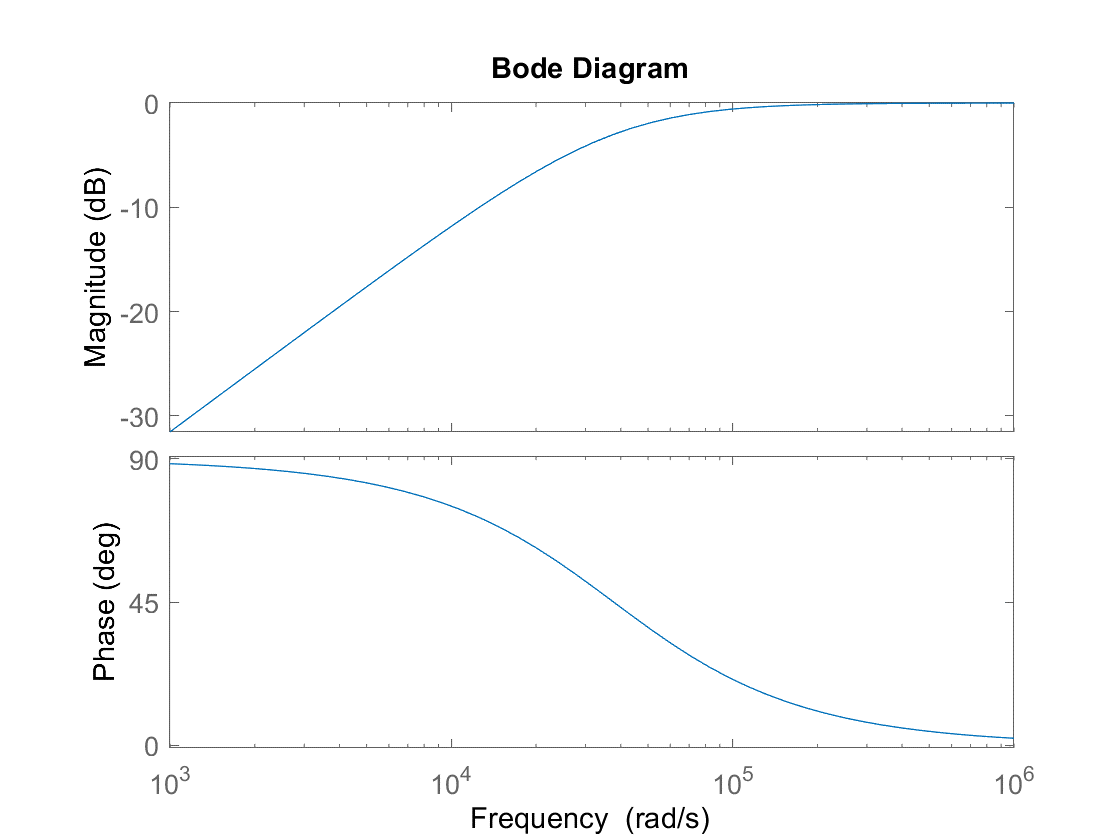
\includegraphics[width=5.65in]{questionbank/networks/rl_high_pass_design/v0/bode_plot.png}
\end{center}
\end{answer}
\end{partquestion}

\end{mainquestion}

% Problem 5 - Parallel RLC impedance (17 points)
\clearpage
\Point{parallelrlc}{deriveimpedance}{4}
\Point{parallelrlc}{maxmagnitude}{4}
\Point{parallelrlc}{extremephase}{4}
\Point{parallelrlc}{bodeplots}{5}
\begin{mainquestion}{parallelrlc}{Parallel RLC Impedance}

Consider the current-driven parallel $RLC$ circuit shown to the right.

\begin{center}
    \includegraphics[width=4.7in]{circuit.png}
\end{center}

\begin{partquestion}{deriveimpedance}{Derive the impedance $Z\left(j\omega\right)$ facing the current source. Express your answer explicitly as the sum of the real and imaginary part.}
\begin{answer}
The total impedance facing the current source will be the parallel combination of the individual impedances, as shown below:

\[
Z\left(j\omega\right) = Z_{R} \parallel Z_{L} \parallel Z_{C} = \frac{1}{\frac{1}{Z_{R}} + \frac{1}{Z_{L}} + \frac{1}{Z_{C}}} = \frac{1}{\frac{1}{R} + \frac{1}{j\omega L} + j\omega C} = \frac{1}{\frac{1}{R} + j\left(\omega C - \frac{1}{\omega L}\right)}
\]

We then simplify by multiplying both the numerator and denominator by the complex conjugate of the denominator, as shown below:
\begin{align*}
Z\left(j\omega\right) &= \frac{1}{\frac{1}{R}+j\left(\omega C-\frac{1}{\omega L}\right)}\cdot\frac{\frac{1}{R}-j\left(\omega C-\frac{1}{\omega L}\right)}{\frac{1}{R}-j\left(\omega C-\frac{1}{\omega L}\right)}\\
&=\frac{\frac{1}{R}-j\left(\omega C-\frac{1}{\omega L}\right)}{\frac{1}{R^2}+\left(\omega C-\frac{1}{\omega L}\right)^2}\\
&=\frac{\frac{1}{R}}{\frac{1}{R^2}+\left(\omega C-\frac{1}{\omega L}\right)^2}-j\frac{\left(\omega C-\frac{1}{\omega L}\right)}{\frac{1}{R^2}+\left(\omega C-\frac{1}{\omega L}\right)^2}
\end{align*}
\end{answer}
\end{partquestion}

\begin{partquestion}{maxmagnitude}{At what frequency is the magnitude of the impedance $\left|Z\left(j\omega\right)\right|$ a maximum? What is the phase angle at that frequency?}
\begin{answer}
We find $\left| Z(j\omega) \right|$ as shown below:

\begin{align*}
\left|Z\left(j\omega\right)\right| &= \left|\frac{\frac{1}{R}-j\left(\omega C-\frac{1}{\omega L}\right)}{\frac{1}{R^2}+\left(\omega C-\frac{1}{\omega L}\right)^2}\right|\\
&=\frac{1}{\sqrt{\frac{1}{R^2}+\left(\omega C-\frac{1}{\omega L}\right)^2}}
\end{align*}

We note that maximizing $\left| Z(j\omega) \right|$ is equivalent to minimizing its denominator. By inspection, we can see that the denominator is minimized when $\omega C = \frac{1}{\omega L}$, which occurs at:

\[
\omega_{0} = \frac{1}{\sqrt{LC}}
\]

In other words, this maximum occurs when the capacitive impedance is equal to the inductive impedance, and the total impedance is just $Z\left(j\omega_{0}\right) = R$. From our first equation in part (\cref{prob:parallelrlc:deriveimpedance}), we can find the phase angle:

\begin{align*}
\angle Z\left(j\omega\right) &= \angle \frac{1}{\frac{1}{R}+j\left(\omega C-\frac{1}{\omega L}\right)}\\
&=\angle 1-\angle\left(\frac{1}{R}+j\left(\omega C-\frac{1}{\omega L}\right)\right)\\
&=0-\tan^{-1}\left[\frac{\omega C-\frac{1}{\omega L}}{\frac{1}{R}}\right]\\
&=-\tan^{-1}\left[\omega RC-\frac{R}{\omega L}\right]
\end{align*}

And it follows that at $\omega = \omega_{0} = \frac{1}{\sqrt{LC}}$, we have:

\begin{align*}
\angle Z\left(j\omega_0\right) &= -\tan^{-1}\left[\omega_0 RC-\frac{R}{\omega_0 L}\right]\\
&= -\tan^{-1}\left[\frac{RC}{\sqrt{LC}}-\frac{R\sqrt{LC}}{L}\right]\\
&= -\tan^{-1}\left[\frac{R\sqrt{C}}{\sqrt{L}}-\frac{R\sqrt{C}}{\sqrt{L}}\right]\\
&= -\tan^{-1}0\\
&= 0
\end{align*}

We could also have easily arrived at this answer by noting (see above) that at $\omega_{0}$ the total impedance becomes $Z = R$, which has a phase of 0 because $R$ is just a real number.
\end{answer}
\end{partquestion}

\begin{partquestion}{extremephase}{What is the phase angle of the impedance at zero (DC) and at extremely high frequency? Provide an intuitive explanation based on the behavior of $C$ and $L$ in these extremes.}
\begin{answer}
At very low frequencies (DC), the inductor behaves like a short circuit, which offers the least impedance path for the incoming current $I_{S}$. It is important to note that the resistor still remains a resistor and the capacitor behaves like an open circuit. The effect of this asymptotic behavior is that the impedance, $Z(j\omega) = R \parallel j\omega L \parallel \frac{1}{j\omega C} \approx j\omega L$ is dominated by the inductor (because $j\omega L$ becomes very small). Since $Z(j\omega) \approx j\omega L = \omega Le^{j\frac{\pi}{2}}$, we should observe the phase angle approaches $\lim\limits_{\omega\to0^+}\angle Z(j\omega)=\frac{\pi}{2}=+90^\circ$.

At extremely high frequency, the capacitor behaves like a short, the inductor like an open, and the resistor remains a resistor. Thus, $Z(j\omega) = R \parallel j\omega L \parallel \frac{1}{j\omega C} \approx \frac{1}{j\omega C}$ is dominated by the capacitor (because $j\omega C$ becomes very large). As such, $Z(j\omega) \approx \frac{1}{j\omega C} = \frac{-j}{\omega C} = \frac{1}{\omega C}e^{-j\frac{\pi}{2}}$ and we observe that the phase angle approaches $\lim\limits_{\omega\to\infty}\angle Z(j\omega)=-\frac{\pi}{2}=-90^\circ$.
\end{answer}
\end{partquestion}

\begin{partquestion}{bodeplots}{Let $R = 7\text{ k}\Omega$, $L = 1\text{ mH}$, and $C = 1\text{ nF}$. Create Bode plots for both the magnitude and phase of the transfer function $\frac{V_{\text{out}}}{I_{S}}$. Note that this transfer function is the impedance of the network, so you do not need to re-derive it!}
\begin{answer}
We can use our first equation from part (\cref{prob:parallelrlc:deriveimpedance}) and massage it into a form that MATLAB will like:

\[
Z\left(j\omega\right) = \frac{1}{\frac{1}{R} + \frac{1}{j\omega L} + j\omega C} = \frac{j\omega L}{\left(j\omega \right)^2LC+\frac{j\omega L}{R} + 1}
\]

Using the following simple MATLAB script:

\begin{verbatim}
L=1e-3;
R=7e3;
C=1e-9;
num=[L 0];
den=[C*L L/R 1];
bode(num,den);
\end{verbatim}

We can generate the Bode plots for magnitude and phase of $Z\left(j\omega\right)$:

\begin{center}
    \includegraphics[width=5.25in]{bode_plot.png}
\end{center}
\end{answer}
\end{partquestion}

\end{mainquestion}